\chapter{Introduction} \label{chap::intro}
The problem of \acl{SLAM}, abbreviated as \acs{SLAM}, is addressed as a fundamental problem in mobile robotics and is considered by many to be a prerequisite in truly autonomous robots. SLAM addresses the problem of a mobile robot moving through an unknown environment of which no map is available {\it a-priori}. The robot has to build a map of the environment through onboard sensing and its movements in the environment, both corrupted by noise. The goal of \acs{SLAM} is to construct the map of an environment and path taken by the robot. 

If the map is available {\it a-priori}, estimating the path of the robot would come close to a localization problem and similarly, if the true path of the robot is made available, building a map is relatively a simple task.  However, if both the map and true path of the robot are unknown, correlations arise between the unknowns which constrains localization and mapping to be considered concurrently, and hence the name \acl{SLAM}.

The thesis discusses about impact-based approach to SLAM problem and its associated solutions. The impact-based approach uses minimal sensing modalities to accomplish SLAM and the solution is implemented for a rectilinear environment using Sphero robots, developed by Orbotix Inc. The robot collides with walls of the environment and builds a map using the collision data and odometry information. The collision is detected through changes in accelerometer data and with this information, robot's orientation and odometry can define the pose of the landmark.  This obstacle can represent a point landmark, a line since all the obstacle are straight walls. A map representation has to be defined for associating the measurement information with the map or in simple words, building the map of environment. 

The suitability of a map representation depends primarily upon sensing modalities and operating environment. As a result, there do not exist a generic SLAM solution which can be suited to any environment and sensing modalities and at the same time produce a consistent solution. Hence, an algorithm has to be developed using the odometry and collision measurements to consistently estimate the map of a rectilinear environment and path taken by the robot. Moreover, achieving a SLAM solution using minimal sensing information has been less studied and this thesis provides a scope for it. These objectives had motivated me in the right direction to pursue this thesis.

This chapter provides a short survey of state-of-the-art in the field of SLAM. This chapter begins with the genesis of SLAM (Section~\ref{sec::bg}), providing a short history of early developments in this field. Section~\ref{sec::sp} describes SLAM through an illustrative framework to gain a better understanding of the problem a detailed explanation of SLAM problem. With a good understanding of the problem, Section~\ref{sec::state_art} puts forward the state-of-the-art solutions for the problem from an estimation viewpoint. These sections provide the appropriate background needed to understand the thesis. Section~\ref{sec::thesis_statement} advances the research objectives for this thesis work, followed by Section~\ref{sec::thesis_contributions} laying out the key thesis contributions. Section~\ref{sec::outline} outlines a brief description of the work done in each Chapter of this thesis.

\section{SLAM genesis} \label{sec::bg}
The genesis of the \acs{SLAM} problem arose from two separate concepts, localization and mapping. The problem of localization has been long addressed since the Second World War under the name `Tracking', while the mapping problem has a history from the geodetic mapping and recently, \acs{SLAM} researchers are adopting techniques from the later \cite{agarwalsurvey}. The notion of a robot to concurrently map and localize grew out when probabilistic methods were just beginning to be introduced into both Robotics and \acf{AI}. The \acs{SLAM} problem was first brought up at the 1986 \acf{ICRA} and a number of researchers recognized that consistent probabilistic mapping is very much required to accomplish SLAM.

The researchers initially focussed on assuming a series of approximations to the \acs{SLAM} problem by reducing it to a decoupled localization-mapping problem. The researchers failed to address the convergence properties of the decoupled problem or the steady-state behaviour, and it was widely assumed that the errors in the map would not converge and would rather exhibit a random-walk behaviour.

The solution to SLAM addressed by \cite{dissanayake2001solution} was the first conceptual breakthrough to provide a converging SLAM solution. The main aspect of this work addressed that the correlations between mapping and localization is important and the solution improved as correlations grew. The convergence and solution was detailed in a probabilistic framework and takes the uncertainty explicitly into account. The research from then on focussed mainly on challenges in implementation such as computational efficiency, data-association, nonlinearity, and consistency.

\acs{SLAM} has now turned out to be an essential capability for mobile robots in unknown environments where globally accurate position data (e.g.\ GPS) is not available. In particular, significant promise has been shown for remote exploration, going to places that are too distant \cite{golombek1997overview}, too dangerous \cite{thrun2003system}, or too costly for human access. If robots are to operate autonomously in extreme environments such as abandoned mines or extra-terrestrial navigation, they must be capable of building accurate maps and navigating reliably according to these maps. Even in benign environments such as indoor environments, accurate prior maps are difficult to acquire. The applications of SLAM, listed so far, makes a primary assumption that the environment is static in nature. However, the extension of SLAM to dynamic environments is not straightforward and is more complex. Recent literature \cite{montemerlo2002conditional} has shown SLAM to work in dynamic environments under various assumptions for human-robot interaction.     

\section{SLAM problem} \label{sec::sp}
Before stepping into mathematical formulations of \acs{SLAM}, Example~\ref{slam_exmp} gives an illustration of a general SLAM problem. 
\begin{exmp}
{\it Consider a mobile robot, equipped with a range sensor and an odometry sensor, placed in an unknown environment. The robot has to implement SLAM by exploring the environment using the given sensors.}

A simple environment is taken into consideration which contains three distinct point landmarks as shown in Figure~\ref{slam_example1}. The range sensor provides information about the landmark location in the environment while the odometry sensor is used to track the position of the robot through its movements. The measurements obtained from both the sensors are corrupted with noise, and for simplicity, the uncertainty in the measurement is modelled as a Gaussian. Here the robot is assumed to detect the corresponding landmark from the measurement, but in future, this problem (called as data association) will considered in detail.   
\begin{figure}
\centering
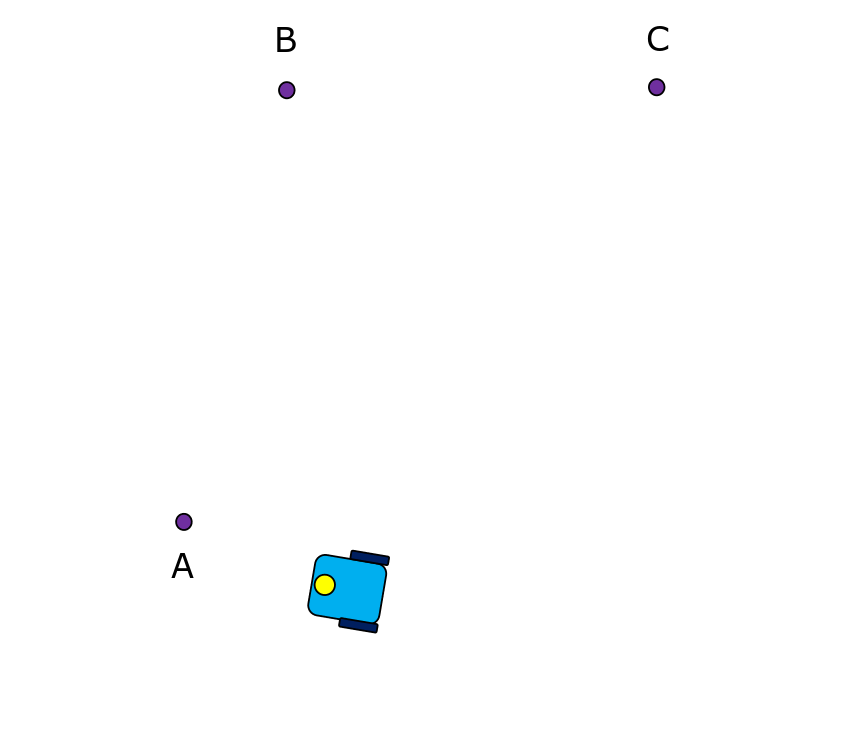
\includegraphics[scale=0.3]{./images/slam_example1}
\caption[Sample environment for a SLAM example]{A simple environment for SLAM\footnotemark}
\label{slam_example1}
\end{figure}
\footnotetext{Courtesy of Margarita Chli for the SLAM example figures}
The robot at its initial location (trivially taken as origin of the map to built), as shown in Figure~\ref{slam_example2}, observes landmark A in its field of view and takes a range measurement. The uncertainty associated with this measurement is represented by an ellipse as shown in Figure~\ref{slam_example3}, which is a 2D Gaussian. 
\begin{figure}
\centering
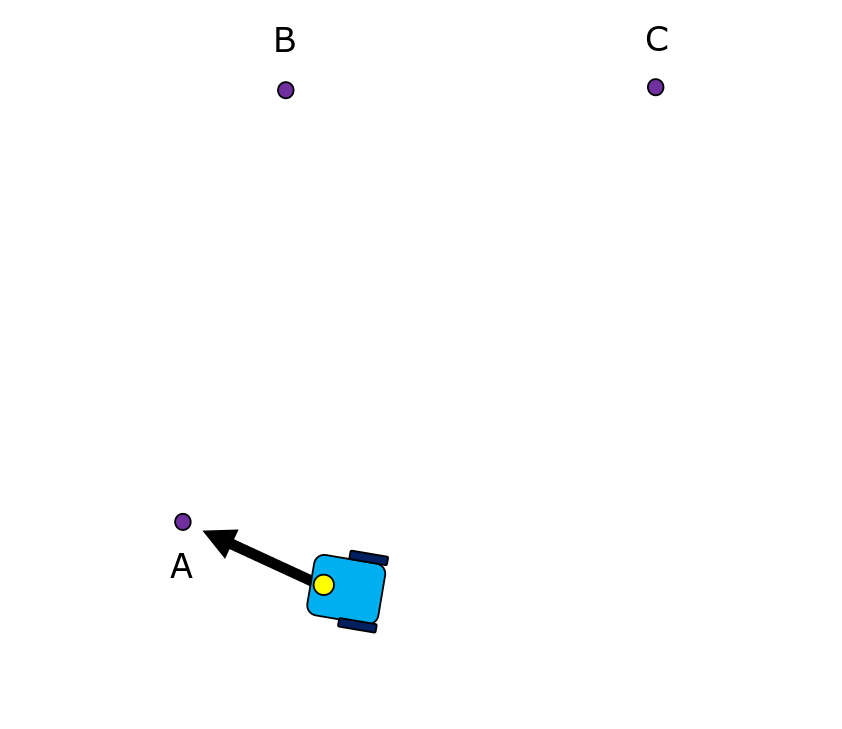
\includegraphics[scale=0.3]{./images/slam_example2}
\caption{First measurement of landmark A}
\label{slam_example2}
\end{figure}
\begin{figure}
\centering
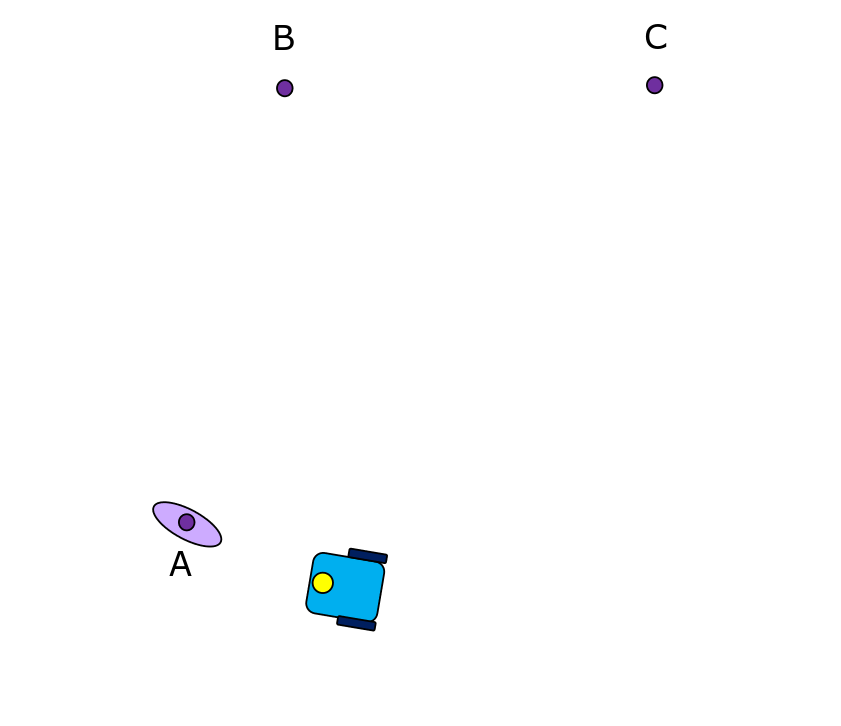
\includegraphics[scale=0.3]{./images/slam_example3}
\caption{Update of landmark position A}
\label{slam_example3}
\end{figure}

The robot begins to explore the environment after the update of landmark A into its memory. The uncertainty associated with its motion measurement from odometry is represented by a similar Gaussian as shown in Figure~\ref{slam_example4}. Due to the uncertainty in the robot's position or the path of the robot, subsequent range measurements of landmarks B and C are corrupted gradually as shown in Figure~\ref{slam_example5} and Figure~\ref{slam_example6}. Hence, the map built through the robot's sensors begin to drift due to this uncertainty.
\begin{figure}
\centering
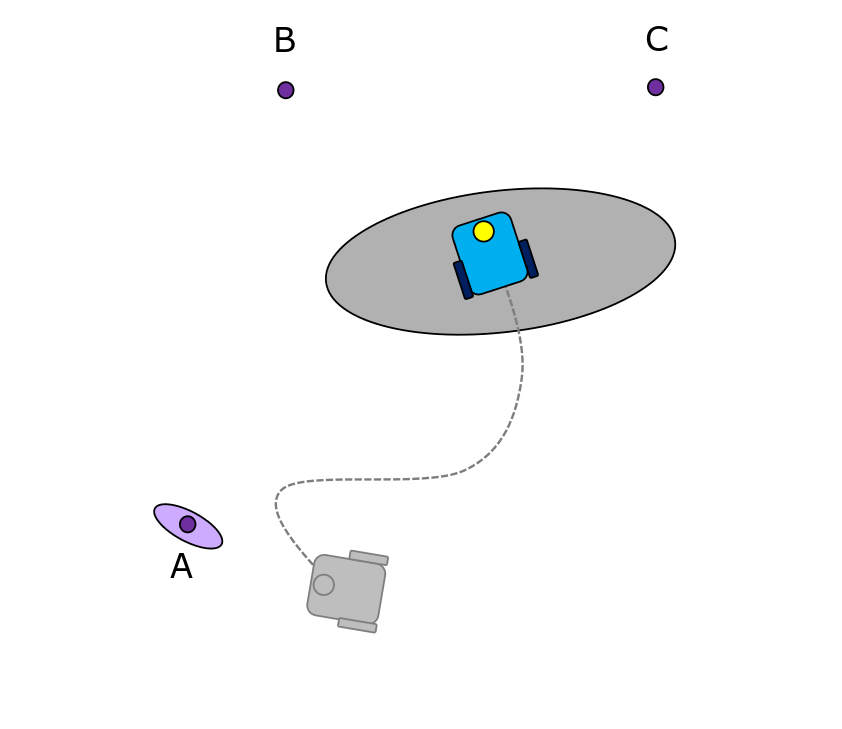
\includegraphics[scale=0.3]{./images/slam_example4}
\caption{Exploration of the environment}
\label{slam_example4}
\end{figure}
\begin{figure}
\centering
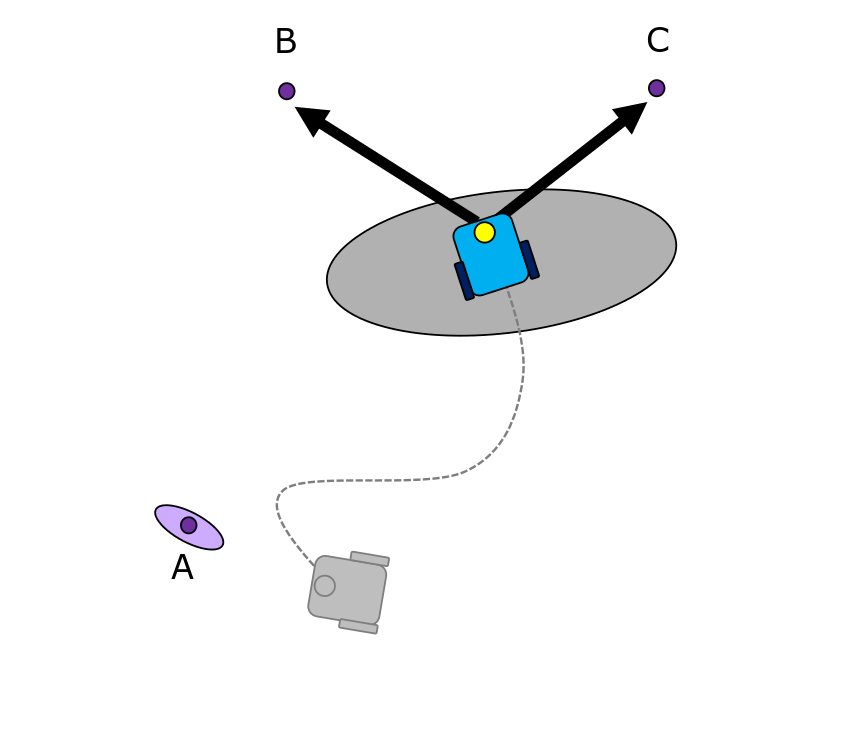
\includegraphics[scale=0.3]{./images/slam_example5}
\caption{Measurements of landmarks B and C}
\label{slam_example5}
\end{figure} 
\begin{figure}
\centering
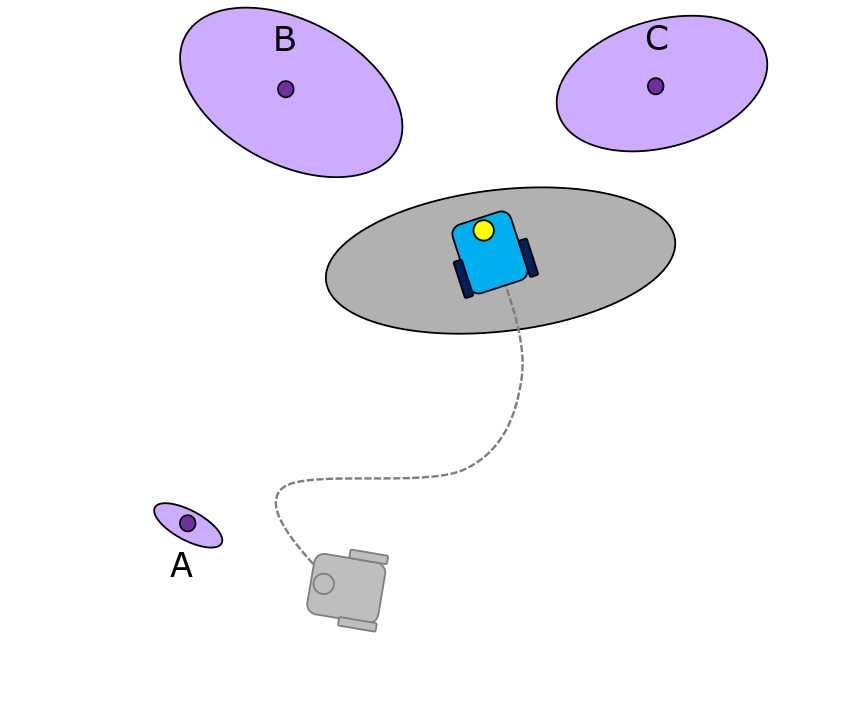
\includegraphics[scale=0.3]{./images/slam_example6}
\caption{Update of landmarks B and C}
\label{slam_example6}
\end{figure} 

The robot continues to explore with the error in the robot position or path begins to grow systematically. At certain point in time, the robot detects an old landmark as shown in Figure~\ref{slam_example8}. The robot compares a new measurement of that landmark with the old measurement and finds a mismatch between them. The main factor contributing to this problem is the error in the robot's current position which is corrected using the new measurement and the old updated estimate of landmark A. Since the entire set of landmark measurements were correlated due to the error in robot's path, all the landmarks get updated as a result. This step is especially called as loop closure problem and it is illustrated in Figure~\ref{slam_example9}.\hfill $\square$

\begin{figure}
\centering
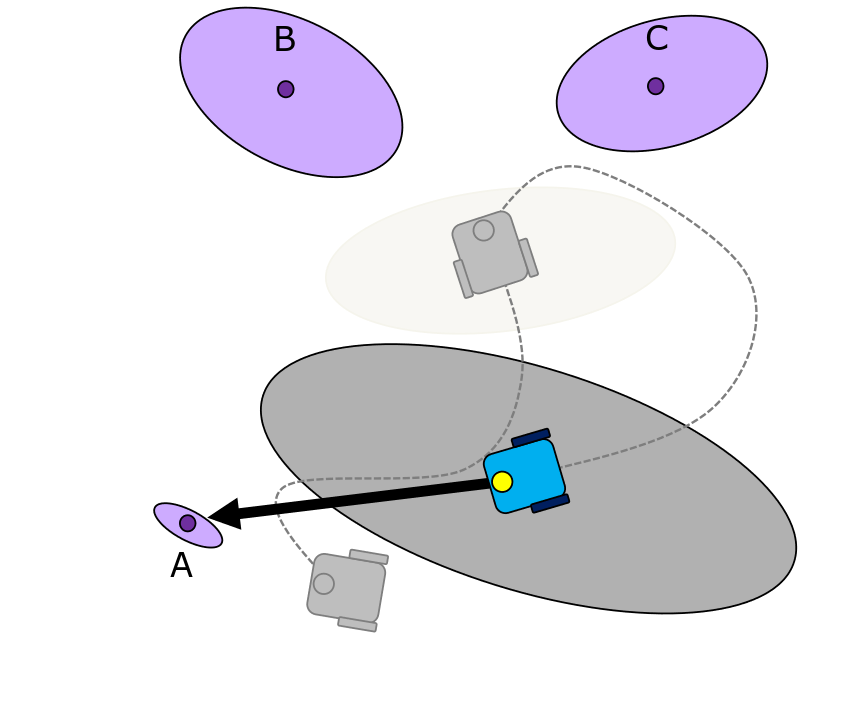
\includegraphics[scale=0.3]{./images/slam_example8}
\caption{Second measurements of landmark A}
\label{slam_example8}
\end{figure} 

\begin{figure}
\centering
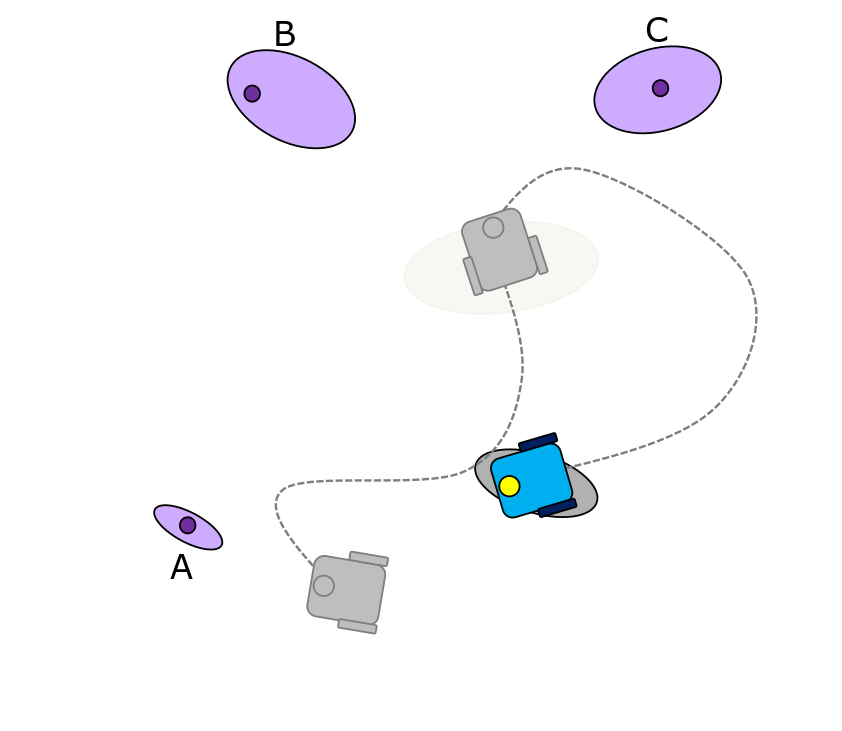
\includegraphics[scale=0.3]{./images/slam_example9}
\caption{Loop closure in SLAM}
\label{slam_example9}
\end{figure}
\label{slam_exmp}  
\end{exmp}

The illustration of \acs{SLAM} makes the problem more clear and gives an intuitive idea. A key factor affecting the estimates of the landmark positions was the error in the robot position or path and this factor bridges a correlation between the landmark estimates and robot position. Moreover, unlike the measurement noise, the error in the robot's pose has a systematic effect on the error in the map and as a result, the true map cannot be estimated without estimating the true path of the robot. This property gives rise to the chicken-egg nature of the SLAM problem. 

A probabilistic formulation of the SLAM problem is used for developing the SLAM algorithm which explicitly deals with the uncertainty in the problem. The probabilistic approach has received wide-spread attention due to their applicability in SLAM and has contributed to a separate dimension in the field of robotics called Probabilistic Robotics \cite{thrun2005probabilistic}. 

According to standard SLAM formulation, a robot executes control and accumulates observations, both corrupted by noise. Each control or observation, coupled with an appropriate noise model, can be thought of as a probabilistic constraint. As the robot explores through the environment, the network of constraints expand and get updated with re-observations. With re-observations, the constraints turn less uncertain and become increasingly rigid. In the limit of infinite observations and controls, the position of all map features become fully correlated. The SLAM problem is illustrated as a network of constraints in Figure~\ref{network_constraint}. For the case of structured environments like the rectilinear environment in the Figure, the landmarks are additionally correlated through geometric structure such as orthogonality.

\begin{figure}
\centering
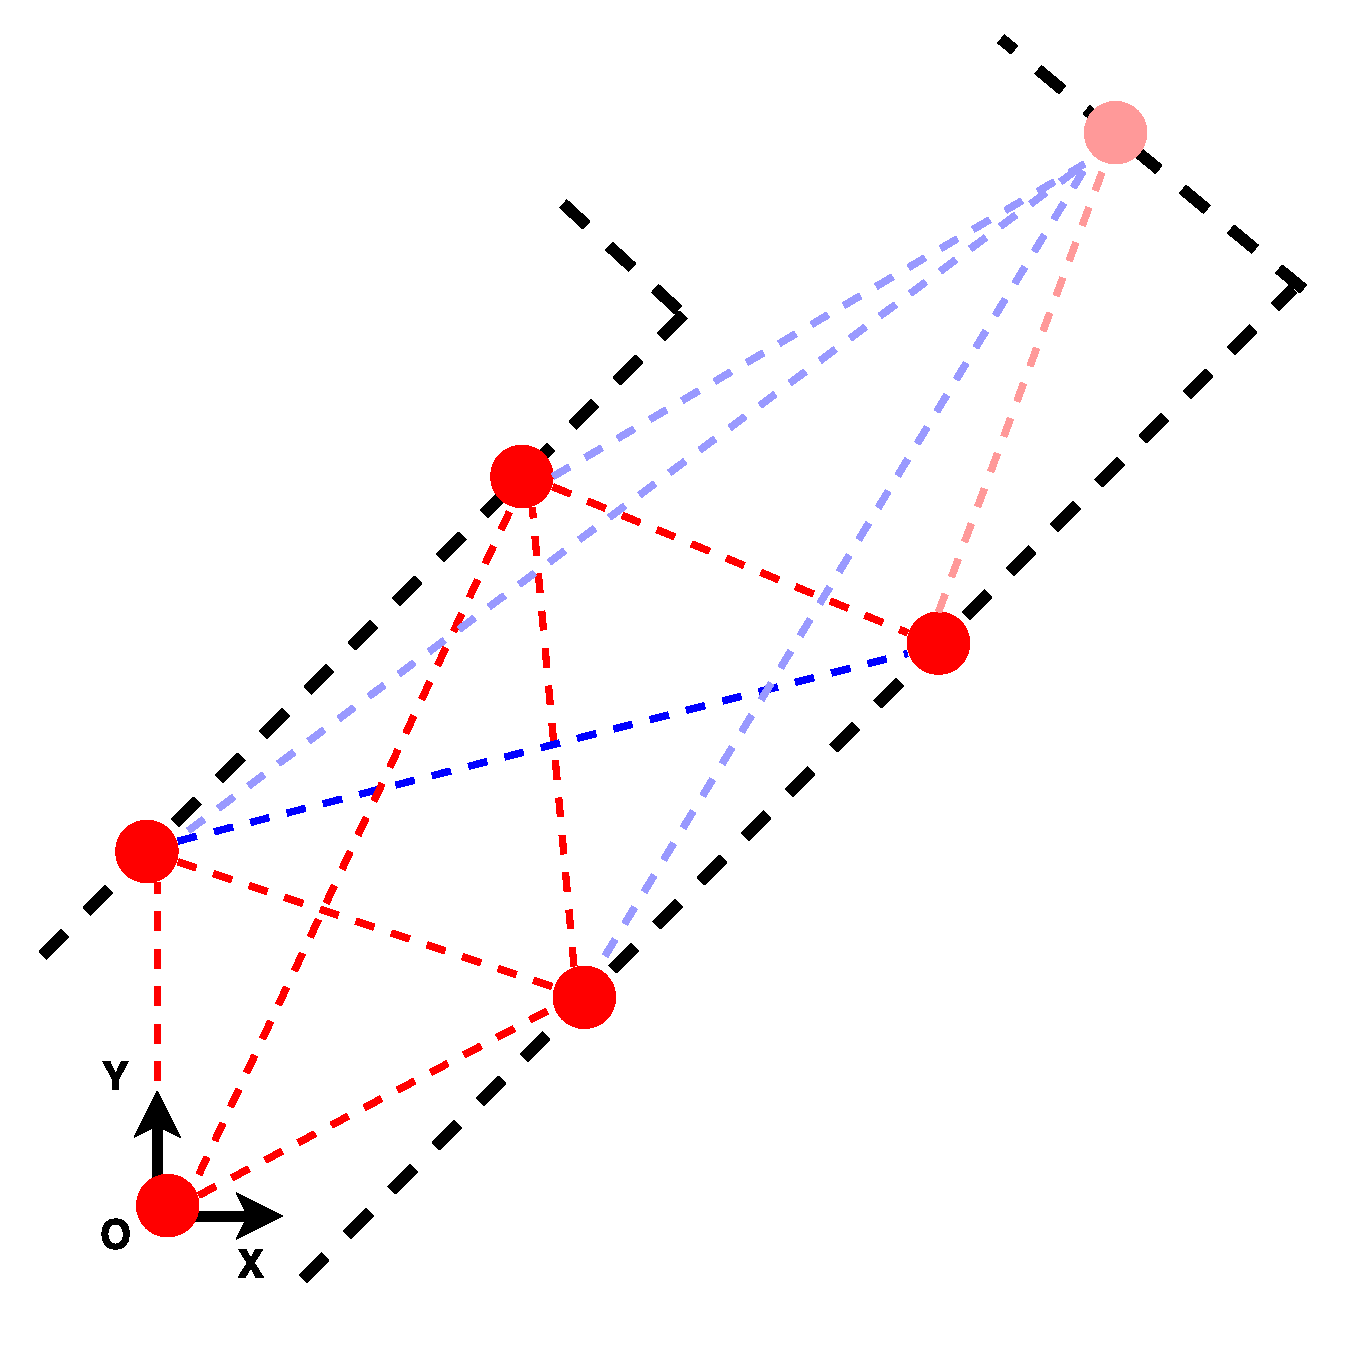
\includegraphics[scale=0.4]{./images/network_constraint}
\caption[Network of constraints in impact-based SLAM]{Network of constraints in impact-based SLAM; multiple observations of landmarks (dark red color) are constrained higher than the new landmarks (light red color). The blue lines represent the correlations through environment structure.}
\label{network_constraint}
\end{figure}  

A popular extension of the above formulation is posterior estimation of the SLAM problem. The objective is to estimate a probability distribution over the possible maps and robot poses, given the observations and controls. The distribution, referred to as SLAM posterior, can be written as:
\begin{equation}
p(s_t,m|z_{1:t},u_{1:t},c_{1:t})
\end{equation}
where \lsymb{$s_t$}{Robot pose at time $t$} is the robot pose at time $t$ and \lsymb{$m$}{Map of an environment} is the map of an environment. The variables \lsymb{$z_{1:t}$}{Time history of observations}, \lsymb{$u_{1:t}$}{Time history of control inputs} and \lsymb{$c_{1:t}$}{Time history of data associations} corresponding to the set of measurements, controls and data associations respectively and the posterior is conditioned upon them. The data association describes the mapping between a measurement $z_t$ and a landmark in $m$. The description of these variables will be explained in detail in the forthcoming chapter.

There does exists an alternative formulation which is suitable for computing the best possible map and robot pose. This approach is commonly called an offline optimization approach where a global nonlinear optimization is carried over a batch of measurements. This approach has gained popularity in the recent years by exploiting the sparsity in SLAM. 

The posterior approach seems desirable since it gives a distribution of possible solutions along with the uncertainty associated with it. This approach is robust in noisy environments since it explicitly considers the uncertainty factor in the problem. At first glance, the optimization approach might seem simpler than the posterior approach, however by considering judicious assumptions about how the state of the world and robot evolves, the posterior computation can be more efficient. For example, consider the following recursive formula, known as Bayes filter, which computes the posterior at time $t$.
\begin{equation}
\begin{split}
p(s_t,m|z_{1:t},u_{1:t},c_{1:t})\,&=\,\eta\,p(z_t|s_t,m,c_t)\cdot \\
&\cdot\int p(s_t|s_{t-1},u_t)\,p(s_{t-1},m|z_{1:t-1},u_{1:t-1},c_{1:t-1})ds_{t-1} 
\end{split}
\label{bayes_filter}
\end{equation}

The above integrand cannot be computed in closed form for a general probability distribution. However, if a particular form of distribution is considered such as Gaussian, a closed loop solution is indeed possible. Variants of Bayes filter such as Kalman filter and Particle filter are discussed in forthcoming section.  

\section{State-of-the-Art solutions} \label{sec::state_art}
Achieving a solution to the SLAM problem was one of the most demanding research in mobile robotics literature for past two decades. SLAM has been regarded as a prerequisite for a robot to be truly autonomous and from decades of research, a practical solution is found to be indeed possible. 

A consistent solution is achieved only when a complete set of correlations are propagated through a sequence of measurements and controls. However, the efficiency of computation ($\mathcal{O}(n^2)$, $n$ being the state dimension) became an obstacle for achieving a practical solution. Researchers \cite{montemerlo2002conditional} later came up with more robust SLAM algorithms which are practically efficient in terms of computational and memory requirements through exploitation of structure in SLAM. This estimation technique is called as online estimation since measurements are processed as they arrive.

The two state-of-the-art approaches for SLAM using online estimation techniques are Extended Kalman Filter-SLAM and Particle filter-SLAM. The two approaches are formulated and discussed in the following sections.

\subsection{Extended Kalman filter-SLAM} \label{sec::ekfslam}
\acf{EKF} is a parametrized representation of Bayes filter which approximates SLAM posterior as a multivariate Gaussian distribution over all features in the map and robot pose. The parametrized representation describes the probability distribution uniquely using mean $\mu$ and covariance $\Sigma$.

The state transition probability is described using the motion model of the robot,
\begin{equation}
p(s_t|s_{t-1},u_t)\Longleftrightarrow s_t~=~f(s_{t-1},u_t)~+~w_t,
\end{equation}
where \lsymb{$f(\cdot)$}{State transition model} corresponds to the robot's motion model, $s_t$ and $u_t$ represent the robot pose and control input respectively at time instant \lsymb{$t$}{Continuous time index}, and \lsymb{$w_t$}{Process noise} represents an additive, zero-mean, uncorrelated Gaussian noise with covariance \lsymb{$Q_t$}{Process noise covariance at time $t$}.

In a similar manner, the observation model is described using the following form-
\begin{equation}
p(z_t|s_t,m)\Longleftrightarrow z_t~=~h(s_t,m)~+~v_t,
\end{equation}
where \lsymb{$h(\cdot)$}{Observation model} describes the geometry of the observation, $z_t$ denotes observation and \lsymb{$v_t$}{Observation noise} represents another additive, zero-mean, uncorrelated Gaussian noise with covariance \lsymb{$R_t$}{Observation noise covariance}.

The state vector for EKF-SLAM  is usually defined as an augmented state of robot pose $s_t$ and observed landmarks $m$. For the observation of a new landmark, a new state is defined using the inverse of observation model, and then append to the original state vector. A feature-based representation is used here where the individual observed point landmarks are defined either through their location or pose. Hence, a map is represented as a set of landmark positions or poses, $m=\begin{bmatrix}m_1, m_2, \cdots, m_N\end{bmatrix}$. Additional details on map representation will be discussed in Section \ref{sec::env_rep}.

The standard EKF method can be applied to compute the mean \gsymb{$\mu_t$}{Mean of state estimate at time $t$} and the covariance \lsymb{$P_t$}{Covariance of state estimate at time $t$} given the measurements $z_{0:t}$ using a recursive update as shown below.

\textbf{Prediction step}
\begin{align}
\hat{s}_{t|t-1}&=f(\hat{s}_{t-1|t-1},u_t) \\
P_{t|t-1}&=\nabla f\cdot P_{t-1|t-1}\cdot\nabla f^T~+~Q_t
\end{align}
The gradient $\nabla f$ is the Jacobian of $f$ evaluated at the estimate $\hat{s}_{t-1|t-1}$.

\textbf{Update step}
\begin{align}
\begin{bmatrix} \hat{s}_{t|t} \\ \hat{m}_t \end{bmatrix}&=\begin{bmatrix} \hat{s}_{t|t-1} \\ \hat{m}_{t-1} \end{bmatrix}+K_t\cdot\left(z_t-h(\hat{s}_{t|t-1},\hat{m}_{t-1})\right) \\
P_{t|t}&=P_{t|t-1}-K_t\cdot S_t\cdot K^T_t \\
S_t&=\nabla h\cdot P_{t|t-1}\cdot \nabla h^T+R_t \\
K_t&=P_{t|t-1}\cdot\nabla h^T\cdot S^{-1}_t
\end{align}

The Kalman gain is denoted by \lsymb{$K_t$}{Kalman gain at time $t$} and innovation covariance is denoted by \lsymb{$S_t$}{Innovation covariance at time $t$}. The Jacobian \gsymb{$\nabla(\cdot)$}{Jacobian of a function} is evaluated with respect to state estimates at respective time instance. 

The above SLAM algorithm assumes that the correspondences of all the landmarks are known prior. SLAM algorithm with unknown correspondences will be detailed in Section \ref{sec::da}, which is a small addition to the existing EKF-SLAM algorithm. Moreover, it is assumed here that all the landmarks are initialized prior.

The prediction step propagates the mean and covariance of the belief in accordance to the motion model. This propagation step only affects the belief distribution associated with the robot pose. The landmarks of the map retain the same mean and covariance due to the static world assumption. 

In the update step, the observed landmark is updated using the innovation and Kalman gain. The Kalman gain is a matrix of size 3 by 3$N$+3, \lsymb{$N$}{Number of landmarks} being the number of landmarks. This matrix is usually not sparse and the information is propagated through the entire state estimate. The fact that the Kalman gain is fully populated for all state variables and not just for the observed landmark and robot pose is because of the correlations, that is observing the landmark does not just improve the position estimate of this very landmark but all the other landmarks as well. The situation is neatly depicted through the Example~\ref{slam_exmp}. Issues such as convergence, computational efficiency and data association have been addressed extensively in literature and a good survey discussing these issues is \cite{bailey2006simultaneous}. The issues specific to impact-based SLAM problem is discussed in Section~\ref{sec::challenges}.

\subsection{Particle filter-SLAM} \label{sec::pfslam}
With the above parametric form of estimation, a closed-form solution is obtained for SLAM. However, various issues such as computational efficiency and data association raised questions of implementing EKF-SLAM for large-scale environments. Meanwhile, the success of non-parametric estimation techniques such as particle filters and its variant, \acf{MCMC} have emerged as a core algorithm in Machine Learning. The direct applicability of particle filter to SLAM is intractable (Remark~\ref{pf_scale}) since they are subjected to the curse of dimensionality and a straightforward implementation of particle filter algorithm will be intractable due to the huge number of variables involved in the map. 
\begin{rem}
The computational requirement scales exponentially with the number of dimensions in a particle filter, as opposed to quadratic scaling of computations for a Gaussian update in an EKF. 
\label{pf_scale} 
\end{rem}

The conceptual breakthrough in the success of particle filters in SLAM was developed by \cite{montemerlo2002fastslam}. The probabilistic Markov chain property and conditional independence were best exploited in implementing a tractable version of particle filter-SLAM. Specifically, the full SLAM problem with known correspondences possess a conditional independence property between any two disjoint set of features in the map, given the robot trajectory. In other words, if the robot trajectory is known to be accurate, the features or landmarks can be estimated independently. The correlation property stressed through the covariance matrix in Gaussian filters is exploited here as a conditional independence relation. This structural observation will make it possible to apply a specific version of particle filters known as \acf{RBPF} to the SLAM problem. The RBPF version will be hereby simply addressed as particle filter-SLAM. The effect of this exploitation brings the tractability to the problem. Note that bringing tractability through approximation has their own downsides. For example, particle resampling will have a long term effect on the consistency of the filter \cite{bailey2006consistency} since the process noise (robot pose error) correlates the landmark estimates unlike standard estimation techniques where the error fades out with incorporation of measurements.

A naive implementation of the RBPF-SLAM requires $\mathcal{O}(MN)$ time, where $M$ is the number of particles in the filter and $N$ is the number of landmarks. A tree-based data structure of landmark representation can reduce the time complexity and memory requirements from linear scale to logarithmic scale $\mathcal{O}(M\log N)$, making it significantly faster than the state-of-the-art EKF-SLAM algorithm \cite{huang2011observability}. This had led to the success of particle filter-SLAM for a real-time implementation in large environments, and its contribution to Stanley car, DARPA \cite{thrun2006stanley}. Another useful property of particle filter-SLAM is data association decisions which is made on per-particle basis rather than the most likely particle. As a result, the particle filter can maintain posterior over multiple associations and helps approximating the full posterior $p(s_{1:t},m,c_{1:t}|z_{1:t},u_{1:t})$. This property of RBPF-SLAM makes it robust towards data association errors. 

Apart from the above favourable properties, ability of particle filter to represent an arbitrary distribution is a generic property and can be usefully exploited here. A non-Gaussian distribution can be easily represented through samples, and hence nonlinear motion models can be easily implemented even in situations when the pose uncertainty is known to be very high. 

Assuming a SLAM posterior distribution with known correspondences, the SLAM problem can be formulated as a joint posterior,
\begin{equation}
p(s_{1:t},m|z_{1:t},u_{1:t})
\end{equation}

The assumption of known correspondences takes into account of perfect data association decisions taken \textit{a-priori}. In case of unknown correspondences, the joint posterior includes another variable $c_{1:t}$ which is estimated using data association techniques. 

The full SLAM posterior can be factorized based on the conditional independence property or Rao-Blackwellization.
\begin{equation}
p(s_{1:t},m|z_{1:t},u_{1:t},c_{1:t})=p(s_{1:t}|z_{1:t},u_{1:t},c_{1:t})\cdot\prod_{n=1}^N p(m_n|s_{1:t},z_{1:t},u_{1:t},c_{1:t})
\label{rbpf_fastslam}
\end{equation}

This factorization leads to a problem of estimating posterior over the robot path and $N$~problems of estimating $N$~landmark locations conditioned on the robot trajectory. The factorization is exact and it is based on the assumption that the robot trajectory is known to be accurate. The independence assumption also holds valid when the landmarks are randomly placed in the environment or the environment is unstructured. The factorization in the particle filter-SLAM is illustrated in Figure~\ref{FastSLAM_DBN}.
\begin{figure}
\centering
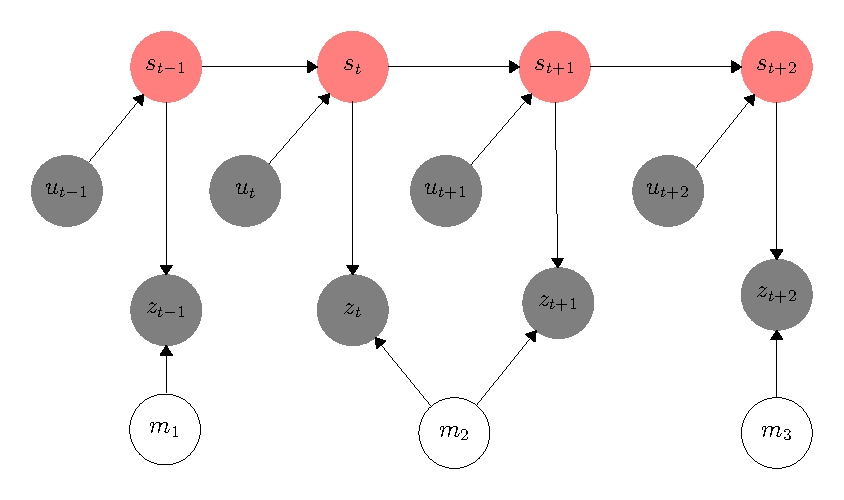
\includegraphics[scale=0.9]{./images/fsm}
\caption[Dynamic Bayesian Network graph of SLAM]{SLAM problem as a Bayes network graph. The control and measurements (gray shaded nodes) render conditional independence in mapping once the entire robot path (red shaded nodes) is known.}
\label{FastSLAM_DBN}
\end{figure}

The path estimate $p(s_{1:t}|z_{1:t},u_{1:t},c_{1:t})$ can be computed efficiently from the sample space since a good approximation of the posterior can be found even in the presence of nonlinear motion models. The landmarks are separately estimated using low dimensional EKFs, and since the landmark estimates are conditioned on the robot path, each particle in the particle filter has its own map of landmark estimates.

The particle filter-SLAM algorithm maintains a set of particles, $Y_t$, of size $M$ and the $k^{\text{th}}$ particle is denoted as $Y_t^{[k]}$. The $k^{\text{th}}$ particle is described systematically as a robot pose (or path) estimate $s^{[k]}_t$ augmented with a set of Gaussian feature estimates as shown below. 

\begin{equation}
Y_t^{[k]}=\left\langle s_t^{[k]}, \mu_{1,t}^{[k]}, \Sigma_{1,t}^{[k]}, \dots, \mu_{N,t}^{[k]}, \Sigma_{N,t}^{[k]} \right\rangle
\label{psf}
\end{equation}  

\textbf{Path estimation}

The particle filter-SLAM samples a new pose $s_t$ in accordance with the $k^{\text{th}}$ particle from the motion model,
\begin{equation}
s_t^{[k]}\sim p(s_t|s_{t-1}^{[k]},u_t)
\end{equation}
where $u_t$ is the current control action and $s_{t-1}^{[k]}$ is the posterior estimate of the robot pose at time $t-1$, residing in the $k^{\text{th}}$ particle. The resulting sample is appended to a temporary particle set which contains the propagated particles at time $t$.

As the previous particle set $Y_{t-1}$ is distributed according to the posterior at $t-1$, the temporary particle set is distributed according to $p(s_t|z_{t-1},u_t,c_{t-1})$. This distribution is referred to as proposal distribution in particle filter. 

After generating $M$ new particles this way, the new posterior set $Y_t$ is obtained from the temporary set by drawing particles (with replacement) with a probability proportional to its importance weight,
\begin{equation}
w_t^{[k]}=\frac{\text{target distribution}}{\text{proposal distribution}}=\frac{p(s_t^{[k]}|z_{1:t},u_{1:t},c_{1:t})}{p(s_t^{[k]}|z_{t-1},u_t,c_{t-1})}.
\label{imp_wt}
\end{equation}     
 
The importance weights for all the particles account for the mismatch between the proposal and the target distribution. This can be illustrated in Figure~\ref{sample_weighting}. The exact calculation of this importance weight will be discussed below. 
\begin{figure}
\centering
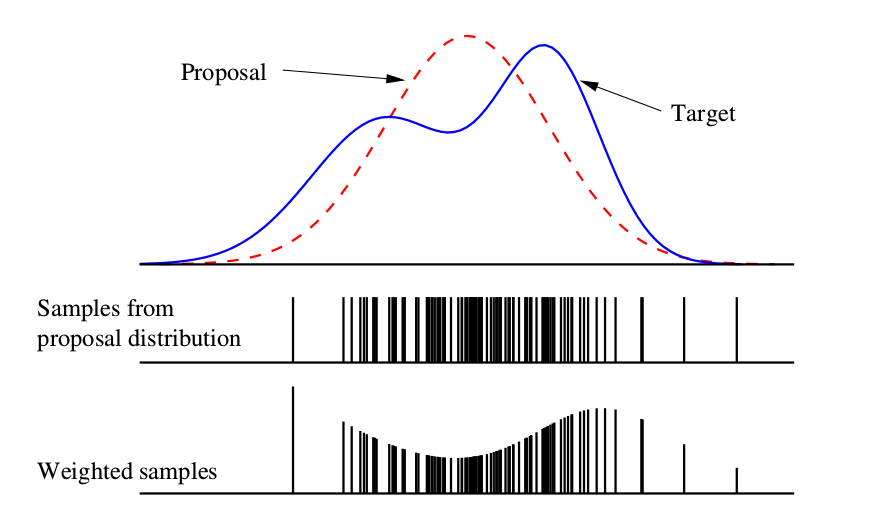
\includegraphics[scale=0.4]{./images/sample_weighting}
\caption[Importance Sampling in a particle filter]{Importance Sampling step in a particle filter \cite{thrun2005probabilistic}}
\label{sample_weighting}
\end{figure}

Note that only the latest pose estimate is used to compute the future posterior in Equation~\ref{imp_wt} according to Markov assumption (see Definition~\ref{def1}). The improvement in computational efficiency as a result of this assumption will be seen in the forthcoming chapter.

\textbf{Landmark location estimation}

From the particle description (\ref{psf}), each particle maintains a set of Gaussians (mean and covariance estimate) for landmarks in the map. For planar environment with point landmarks, the mean $\mu_{i,t}^{[k]}$ is a 2-element vector and the covariance $\Sigma_{i,t}^{[k]}$ is a $2\times 2$ matrix for a landmark. These variables are propagated with the incoming measurements.

For a landmark whose correspondence does not relate to the measurement, the corresponding Gaussian is unchanged.
\begin{equation}
\left\langle \mu_{i,t}^{[k]}, \Sigma_{i,t}^{[k]} \right\rangle=\left\langle \mu_{i,t-1}^{[k]}, \Sigma_{i,t-1}^{[k]} \right\rangle
\end{equation}

Otherwise, the corresponding Gaussian is updated using Bayes' product.
\begin{equation}
p(m_{c_t}|s_{1:t},z_{1:t},c_{1:t})=\eta\cdot p(z_t|s_t,m_t,c_t)\cdot p(m_{c_t}|s_{1:t-1},z_{1:t-1},c_{1:t-1})
\label{bayes_produp}
\end{equation}    

This update is implemented using an EKF where the observation model $z_t=h(s_t,m)$ is linearized at the current system state.

\textbf{Calculation of importance weights}

The problem of calculating the importance weights is continued from (\ref{imp_wt}) as follows,
\begin{align}
w_t^{[k]}&\propto\frac{p(s_t^{[k]}|z_{1:t},u_{1:t},c_{1:t})}{p(s_t^{[k]}|z_{t-1},u_t,c_{t-1})} 
\\
\intertext{From Bayes' product,}
&\propto p(z_t,c_t|s_t^{[k]},z_{1:t-1},u_{1:t},c_{1:t-1}), \\
\intertext{and using Markov assumption,}
&\approx\int p(z_t|m_i^{[k]},s_t^{[k]},c_{1:t})\cdot p(m_i^{[k]})\cdot dm
\end{align}

The above integral can be computed as a finite sum due to a discrete representation of a map. The probabilities can be convolved as Gaussians using a linearized observation model and a Gaussian posterior of the map. For a detailed proof of the importance weight calculation, refer~\cite{montemerlo2002fastslam}.

In the above formulation, the particles are sampled according to the motion model using the current control input and then weighted according to its likelihood with the incoming measurement. The particles are then resampled to obtain the posterior distribution. One of the practical issues in SLAM is degeneracy in evolution of posterior distribution over time. The degeneracy is observed in a scenario where the motion model is less accurate as compared to the observation (measurement) model. The proposal distribution using the less accurate motion model generates a large spectrum of samples (or particles) out of which a small subset has a high likelihood with the incoming measurements. After resampling, only few particles from the proposal distribution survive after resampling (see Figure~\ref{fastslam2}) and this can result in loss of particle diversity or degeneracy. The state-of-the-art version of particle filter-SLAM, \cite{montemerlo2007fastslam}, avoids this problem by incorporating measurements into the motion model for a better prediction estimate, at the expense of intensive computation.
\begin{figure}
\centering
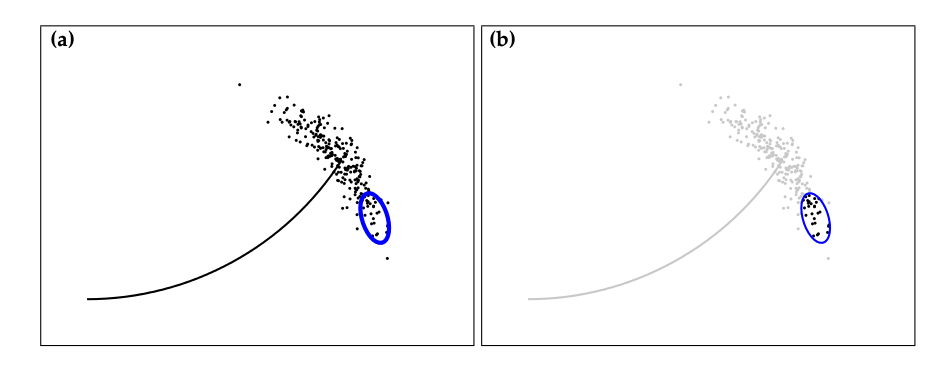
\includegraphics[scale=0.4]{./images/fastslam2}
\caption[Modified proposal distribution for SLAM]{(a) Mismatch between proposal and posterior distribution, and (b) the contribution of samples after resampling \cite{thrun2005probabilistic}.}
\label{fastslam2}
\end{figure}

\section{Research objectives} \label{sec::thesis_statement}
With the appropriate introduction, the thesis work will focus on a minimalistic approach to achieve \acl{SLAM}. The main research problem for the thesis is to accomplish SLAM with an impact-based approach using minimal sensing information. 

In this dissertation, I will advance the following thesis:
\begin{center}
\noindent\parbox{0.9\textwidth}{\it An impact-based approach to Simultaneous Localization and Mapping with minimal sensing information is proposed and implemented.}
\end{center}

The feature extraction in impact-based SLAM is sparse in nature and it may require a long exploration to map the environment. For example, an omnidirectional camera requires a single frame of data to map a simple rectangular environment while it may take many collisions for the impact-based approach. The thesis work is extended to use multiple robots to map the environment and merge the individual maps from the robots. This map-merging problem has a short exploration time and can also ensure a more consistent map of the environment.

\section{Thesis contributions} \label{sec::thesis_contributions}
In this thesis, a probabilistic formulation of the impact-based SLAM problem is addressed with a suitable robot model and an environment representation. A unicycle motion model is used to approximate the robot motion in the environment with the effect of collisions on robot motion modelled through a Finite State Machine, and a suitable rectilinear environment representation is used for incorporating measurements from the environment. 

\begin{center}
{\it A new efficient map representation is proposed for rectilinear environments.}
\end{center}

The new representation models walls of a rectilinear environment as histograms and this representation is compared with the traditional point landmark representation. The new representation might share a similarity with occupancy maps since both involve discretizing the state space. However, the new map representation rasterizes only the useful part (for recording collision measurements) of the map, thereby giving it an edge over the occupancy maps in terms of memory usage and consistency. The suitability and efficiency of map representation is addressed in detail along with an implementation of the most suitable one.

\begin{center}
{\it \centering The impact-based SLAM algorithm is developed using probabilistic formulation and is implemented on the practical setup.}
\end{center}

An impact-based SLAM algorithm is developed using the robot and environment model with collision and odometry information as inputs and robot's path and map as outputs. A particle filter-SLAM is preferred over the existing state-of-the-art SLAM algorithms due to favourable properties relating to the impact-based mapping as follows. Firstly, the poor pose distribution of the robot can be easily represented through a set of particles rather than a smooth Gaussian representation. Secondly, the growth of map information can be well represented through a discrete distribution because of the availability measurement information.
 
A clear layout is made for the impact-based SLAM algorithm detailing the key steps for obtaining the solution. Simulation results validate the feasibility of SLAM solution and comparisons between various landmark representations are analysed. Issues such as convergence, computational effort and consistency of the solution are addressed. The impact-based SLAM algorithm is implemented on a practical setup using Sphero robot and is extended to multiple robot-SLAM. 

\begin{center}
{\it The SLAM problem is accomplished with multiple robots as a map-merging problem for achieving a higher consistency.}
\end{center}

The robots individually build a local map of the environment and at some point, the maps are fused together which has a higher consistency than the single robot-SLAM and is achieved with a lower exploration time.

\section{Outline} \label{sec::outline}
This thesis report comprises of five chapters, including the current chapter. Chapters~\ref{chap::problem}~and~\ref{chap::solution} give the necessary theoretical background for impact-based SLAM with simulation results, followed by Chapter~\ref{chap::implementation} implementation of the developed algorithm. Chapter~\ref{chap::conclusion} summarizes the thesis with a discussion and recommendations for future work. 

A detailed outline of the thesis is as follows,

\textbf{Chapter~\ref{chap::problem}} formulates SLAM in a probabilistic fashion suitable for impact-based SLAM. The motion model and observation model is defined for the impact-based approach along with a suitable environment representation. Various challenges to the SLAM problem are addressed.

\textbf{Chapter~\ref{chap::solution}} presents an impact-based SLAM algorithm using Rao-Blackwellized particle filter. Suitable illustrations and simulation results support the developed algorithm, followed by map-merging problem using multiple robots.

\textbf{Chapter~\ref{chap::implementation}} provides the results of SLAM experimentation with Sphero robots. The robot and its sensing modalities are discussed. The experimental results for both single robot and multiple robot-SLAM are provided.

\textbf{Chapter~\ref{chap::conclusion}} summarizes the thesis with a discussion and recommendations for future work.  